% !TeX program = lualatex
% !TeX encoding = utf8
% !TeX spellcheck = uk_UA
% !BIB program = biber

\documentclass[]{beamer}
\usetheme{PlasmaPhysics}
\usepackage{PlasmaPhysics}
\graphicspath{{pictures/}}

\begin{document}
%==============================================================================================



% --- Слайд 2 ---
\begin{frame}{Закон Бугера–Ламберта–Бера}
    \begin{equation*}
        I(\nu) = I_0(\nu) \cdot e^{-\mu(\nu) \cdot l}
    \end{equation*}
    \begin{itemize}
        \item \( \mu(\nu) \) — коефіцієнт поглинання при частоті \( \nu \) \([\text{см}^{-1}]\)
        \item \( l \) — довжина шляху світла в зразку (см)
        \item У логарифмічній формі:
        \[
        A(\nu) = \log_{10}\left( \frac{I_0}{I} \right) = \varepsilon(\nu) \cdot c \cdot l
        \]
        \item \( \varepsilon(\nu) \) — молярний коефіцієнт екстинкції \(\left[\frac{\text{л}}{\text{моль} \cdot \text{см}}\right]\)
    \end{itemize}
\end{frame}

% --- Слайд 1 ---
\begin{frame}{Як досліджують ІЧ-спектри}

\begin{center}
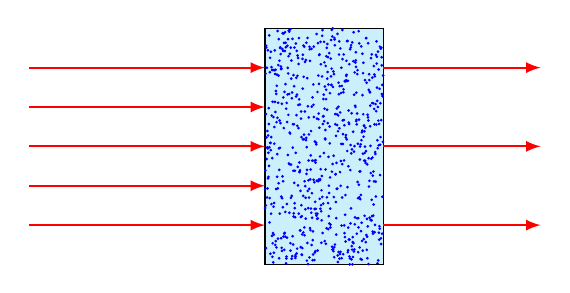
\begin{tikzpicture}[>=latex]

% Зразок
\fill[cyan!20, draw=black] (3,0) rectangle ++(1.5,3);
\draw[] plot [only marks, mark=*, mark size=0.25, mark options={color=blue}, domain=3:4.5, samples=700] (\x,{rnd*3});



% Промені вхідні
\foreach \y in {0.5, 1, ...,2.5} {
  \draw[->, thick, red] (0,\y) -- (3,\y);
}

% Промені вихідні (менше)
\foreach \y in {0.5,1.5,...,2.5} {
  \draw[->, thick, red] (4.5,\y) -- ++(2,0);
}

\end{tikzpicture}
\end{center}
    \begin{itemize}
        \item Джерело інфрачервоного випромінювання створює інтенсивність \( I_0(\nu) \).
        \item Це випромінювання проходить через зразок, і на виході реєструється \( I(\nu) \).
        \item Ослаблення сигналу на частоті \( \nu \) пов'язане з поглинанням світла молекулами.
        \item Вимірюється відношення \( \frac{I(\nu)}{I_0(\nu)} \), що несе інформацію про енергії коливальних переходів.
    \end{itemize}
\end{frame}



% --- Слайд 3 ---
\begin{frame}{Енергія, що поглинається зразком}



    \begin{itemize}
        \item Поглинута енергія на частоті \( \nu \):
        \[
        dE(\nu) = \left[I_0(\nu) - I(\nu)\right] d\nu = I_0(\nu)\left(1 - e^{-\mu(\nu) l}\right) d\nu
        \]
        \item Якщо \( \mu(\nu) \cdot l \ll 1 \), маємо:
        \[
        1 - e^{-\mu(\nu) l} \approx \mu(\nu) l
        \Rightarrow dE(\nu) \approx I_0(\nu) \cdot \mu(\nu) \cdot l \, d\nu
        \]
        \item Підставляємо \( \mu(\nu) = \varepsilon(\nu) \cdot c \):
        \[
        dE(\nu) \approx I_0(\nu) \cdot \varepsilon(\nu) \cdot c \cdot l \, d\nu
        \]
    \end{itemize}
\end{frame}

% --- Слайд 4 ---
\begin{frame}{Сумарна інтенсивність смуги}
    \begin{itemize}
        \item Загальна енергія, поглинута зразком:
        \[
        E_{\text{total}} \propto \int \varepsilon(\nu) \, d\nu
        \]
        \item Визначаємо інтегральну інтенсивність смуги:
        \[
        I = \int \varepsilon(\nu) \, d\nu
        \]
        \item Одиниці виміру:
        \[
        \frac{1000\ \text{см}^2}{\text{моль}} \cdot \text{см}^{-1} = \frac{0.01\ \text{км}}{\text{моль}}
        \]
        \item Це і є величина, яку порівнюють з теоретичними розрахунками.
    \end{itemize}
\end{frame}

% --- Слайд 6 ---
\begin{frame}{Теоретичне визначення \(\varepsilon(\nu)\)}
    \begin{itemize}
        \item \(\varepsilon(\nu)\) визначає ймовірність коливального переходу при частоті \(\nu\)
        \item Пропорційна квадрату перехідного дипольного моменту:
        \[
        \varepsilon(\nu) \propto \left| \left\langle \psi_f \middle| \mu \middle| \psi_i \right\rangle \right|^2 \cdot \delta(\nu - \nu_0)
        \]
        \item У реальних спектрах дельта-функція замінюється профілем (Гауссівським чи Лоренцівським):
        \[
        \varepsilon(\nu) = \varepsilon_{\max} \cdot \text{profile}(\nu - \nu_0)
        \]
        \item Ширина смуги залежить від температури, колізій і розподілу геометрій
    \end{itemize}
\end{frame}


% --- Слайд 7 ---
\begin{frame}{Розрахунок \(\varepsilon(\nu)\) у квантовій хімії}
    \begin{enumerate}
        \item Оптимізується геометрія молекули
        \item Обчислюються нормальні коливання (гармонічні частоти)
        \item Для кожного режиму:
        \[
        \varepsilon \propto \left| \frac{d\vec{\mu}}{dQ} \right|^2
        \]
        — градієнт дипольного моменту по координаті нормального коливання
        \item Результат дається як інтенсивність у \(\frac{\text{км}}{\text{моль}}\) — інтеграл:
        \[
        I = \int \varepsilon(\nu)\, d\nu
        \]
        \item Спектр формується згорткою піків із шириною згладження
    \end{enumerate}
\end{frame}



\end{document}

%            \ifnum\i<4
%            pic[pos=0.35] {upspinarrow}  pic[pos=0.65] {downspinarrow}
%            \fi